% =============================================================================
% CHAPTER 17: DIE EMERGENTE INTERVENTIONSTHEORIE
% =============================================================================
%------------------------------------------------------------------------------
% Chapter 17: Die Emergente Interventionstheorie (Master Chapter)
%------------------------------------------------------------------------------
% Version: 3.1 (January 2026) - Updated cross-references to Ch18-20
%
% Purpose: Master Chapter presenting the emergent theory of interventions.
%          Interventions are not primitive categories but emerge from the
%          continuous 10C space. This chapter establishes the theoretical
%          foundation; heuristics and archetypes follow in Chapter 20.
%
% Primary Appendix: HHH - METHOD-TOOLKIT
% Secondary Appendices: AAA-HI (10C COREs), BBB (Parameters), G (Glossary)
%
% Prerequisites: Chapters 1-16 (complete 10C Framework understanding)
% Leads to: Ch18 (Journey), Ch19 (Segments), Ch20 (Heuristics & Portfolios)
%
% Chapter Type: C (Application)
%
% KEY CHANGE v3.0: Shift from "8 primitive types" to emergent continuous
%                  intervention space. Types are empirical clusters, not
%                  ontological categories.
%------------------------------------------------------------------------------
% =============================================================================

\chapter{Die Emergente Interventionstheorie}
\label{ch:intervention-logic}

%%%%%%%%%%%%%%%%%%%%%%%%%%%%%%%%%%%%%%%%%%%%%%%%%%%%%%%%%%%%%%%%%%%%%%%%%%%%%%%
% CHAPTER SCOPE BOX
%%%%%%%%%%%%%%%%%%%%%%%%%%%%%%%%%%%%%%%%%%%%%%%%%%%%%%%%%%%%%%%%%%%%%%%%%%%%%%%
\begin{tcolorbox}[
    colback=purple!5!white,
    colframe=purple!75!black,
    title={\textbf{Chapter Scope: Ziel / In-Scope / Out-of-Scope}},
    fonttitle=\bfseries
]

\textbf{Ziel (Objective):}
Apply the EBF framework to t1-t8 primitive types, 20-field schema with practical examples and policy implications.

\vspace{0.3cm}
\textbf{In-Scope:}
\begin{itemize}[nosep]
    \item Practical applications of t1-t8 primitive types
    \item Multiple worked examples (≥2)
    \item Policy implications and recommendations
    \item Implementation guidance
\end{itemize}

\vspace{0.3cm}
\textbf{Out-of-Scope (delegiert an Appendices):}
\begin{itemize}[nosep]
    \item Theoretical foundations $\rightarrow$ Foundation chapters
    \item Formal proofs $\rightarrow$ FORMAL appendices
    \item Parameter estimation methods $\rightarrow$ METHOD appendices
\end{itemize}

\end{tcolorbox}



% -----------------------------------------------------------------------------
% QUICK REFERENCE BOX
% -----------------------------------------------------------------------------
\begin{tcolorbox}[colback=blue!5!white, colframe=blue!75!black,
    title=Zentrale Begriffe in diesem Kapitel]
\small
\begin{tabular}{@{}ll@{}}
\textbf{Axiom A0} & Zielgerichtetes Handeln unter Unsicherheit in Kontext \\
\textbf{Emergenz-Kette} & A0 $\rightarrow$ 10C $\rightarrow$ Interventionsraum \\
\textbf{10C-Vektor} & $\vec{I} = (I_{\text{WHO}}, I_{\text{WHAT}}, ..., I_{\text{HIERARCHY}})$ \\
\textbf{Kontinuierlicher Raum} & Interventionen als Punkte/Trajektorien in $\mathbb{R}^n$ \\
\textbf{Emergenter Baukasten} & Kontext-spezifische Intervention aus 10C-Profil \\
\textbf{$I(t)$} & Temporale Trajektorie einer Intervention \\
\end{tabular}
\end{tcolorbox}

% -----------------------------------------------------------------------------
% APPENDIX REFERENCES BOX
% -----------------------------------------------------------------------------
\begin{tcolorbox}[colback=gray!5!white, colframe=gray!75!black,
    title=Appendix-Referenzen]

\textbf{Primär:}
\begin{itemize}[nosep]
\item Appendix UNMAPPED_IE (CORE-EIT): Emergente Interventionstheorie --- Theoretische Grundlagen
\item Appendix TKT (METHOD-TOOLKIT): Operative Umsetzung und LLMMC-Protokolle
\end{itemize}

\textbf{10C COREs (Emergenz-Basis):}
\begin{itemize}[nosep]
\item AAA (WHO), C (WHAT), B (HOW), V (WHEN), BBB (WHERE)
\item AU (AWARE), AV (READY), AW (STAGE), HI (HIERARCHY)
\end{itemize}

\textbf{Unterstützend:}
\begin{itemize}[nosep]
\item III (METHOD-LLMMC-CAL): R-Score und Validierung
\item G (REF-GLOSSARY): Begriffsdefinitionen
\end{itemize}

\textbf{Single Source of Truth:}
\begin{itemize}[nosep]
\item \texttt{docs/frameworks/core-framework-definition.yaml}: 10C SSOT
\end{itemize}

\end{tcolorbox}

% -----------------------------------------------------------------------------
% CROSS-REFERENCE: EMERGE ALGORITHM (Chapter 11, EIT-EMP)
% -----------------------------------------------------------------------------
\begin{tcolorbox}[colback=blue!5!white, colframe=blue!75!black,
    title=\textbf{Cross-Reference: EMERGE Algorithm (Chapter 11, EIT-EMP)}]

Dieses Kapitel etabliert die \textbf{theoretische Grundlage} der Emergenten Interventionstheorie. Der \textbf{EMERGE-Algorithmus} (Kapitel 11) operationalisiert diese Theorie:

\vspace{0.2cm}
\textbf{Theorie (Ch17) → Algorithmus (Ch11):}
\begin{center}
\small
$\vec{I} \in [0,1]^{10}$ (kontinuierlicher Raum) $\xrightarrow{\text{EMERGE}}$ $K^*$ (optimale Anzahl) + Profil $P^*$
\end{center}

\textbf{EIT-EMP Verbindungen:}
\begin{itemize}[nosep]
\item \textbf{EIT-EMP-1 ($\gamma$-Emergence):} Komplementarität emergiert aus $\vec{I}$-Dimension Alignment
\item \textbf{EIT-EMP-2 (K-Optimal):} $K^* = f(\text{budget}, \text{complexity}, \text{stage}, \text{crowding}, \text{scope})$
\item \textbf{EIT-EMP-3 (Scope Levels):} L0→L4 mit Mechanism-Affinity Matrix
\end{itemize}

\vspace{0.2cm}
\textbf{Emergenz-Kette (erweitert):}
\begin{equation*}
\text{A0} \to \text{10C} \to \vec{S}_0 \to \underbrace{\vec{I}}_{\text{Ch17}} \to \underbrace{K^*, P^*}_{\text{Ch11 EMERGE}} \to \underbrace{\text{Portfolio}}_{\text{Ch20}}
\end{equation*}

\vspace{0.2cm}
\textit{Siehe: Chapter 11 §11.20 (EMERGE Algorithm), Appendix UNMAPPED_IE (EMERGE-SPEC)}
\end{tcolorbox}

% -----------------------------------------------------------------------------
% INTUITION BOX
% -----------------------------------------------------------------------------
\begin{tcolorbox}[colback=yellow!5!white, colframe=yellow!75!black,
    title=Intuition: Anna und die unendlichen M\"{o}glichkeiten]

Anna leitet das Pr\"{a}ventionsprogramm einer Schweizer Krankenkasse. Ihr Ziel: Die Diabetes-Pr\"{a}valenz unter 45-65-J\"{a}hrigen um 20\% senken.

Sie steht vor einem klassischen Problem: \textit{Welche Intervention?}

\textbf{Die alte Denkweise:} ``W\"{a}hle aus 8 Interventionstypen den passenden aus.''

\textbf{Die neue Denkweise:} ``Verstehe den Kontext so gut, dass die richtige Intervention \textit{emergiert}.''

Der Unterschied ist fundamental: Statt aus einem Katalog zu w\"{a}hlen, l\"{a}sst Anna die Intervention aus dem spezifischen 10C-Profil ihrer Zielgruppe entstehen. Es gibt keine ``richtige Schublade''---es gibt nur das richtige Verst\"{a}ndnis.

\textit{Am Ende dieses Kapitels wird Anna verstehen, warum Interventionen keine Kategorien sind, sondern Punkte in einem kontinuierlichen Raum---und wie sie f\"{u}r jeden Kontext den passenden Punkt findet.}
\end{tcolorbox}

% -----------------------------------------------------------------------------
% CENTRAL QUESTION BOX
% -----------------------------------------------------------------------------
\begin{tcolorbox}[colback=red!5!white, colframe=red!75!black,
    title=Die Zentrale Frage]
\textbf{Wie emergieren Interventionen aus dem 10C-Framework, und warum ist der Interventionsraum kontinuierlich statt diskret?}

Und spezifischer:
\begin{enumerate}[nosep]
\item Woraus emergieren die 10C-Fragen selbst? (Axiom A0)
\item Wie spannt 10C einen kontinuierlichen Interventionsraum auf?
\item Warum sind ``Interventionstypen'' keine Primitive, sondern emergente Cluster?
\item Wie emergiert f\"{u}r jeden Kontext ein spezifischer Interventionsbaukasten?
\end{enumerate}
\end{tcolorbox}

% -----------------------------------------------------------------------------
% CHAPTER OVERVIEW
% -----------------------------------------------------------------------------
\begin{tcolorbox}[colback=green!5!white, colframe=green!75!black,
    title=Kapitel\"{u}bersicht]

Dieses Kapitel pr\"{a}sentiert die \textbf{emergente Theorie der Interventionen}. Der zentrale Paradigmenwechsel:

\begin{center}
\begin{tabular}{@{}ll@{}}
\textbf{ALT:} & 8 primitive Interventionstypen als fixe Kategorien \\
\textbf{NEU:} & Kontinuierlicher Interventionsraum, der aus 10C emergiert \\
\end{tabular}
\end{center}

\begin{enumerate}
\item \textbf{Teil 0} (Section~\ref{sec:17-status-quo}): \textbf{10C Status Quo Assessment}
    \begin{itemize}[nosep]
    \item Diagnose VOR Intervention
    \item Der 10C Status Quo Vektor $\vec{S}_0$
    \end{itemize}
\item \textbf{Teil I} (Section~\ref{sec:17-axiom}): \textbf{Axiom A0 und die Emergenz-Kette}
    \begin{itemize}[nosep]
    \item Das fundamentale Axiom
    \item Emergenz der 10C-Fragen
    \item Emergenz von FEPSDE und $\Psi$
    \end{itemize}
\item \textbf{Teil II} (Section~\ref{sec:17-continuous}): \textbf{Der kontinuierliche Interventionsraum}
    \begin{itemize}[nosep]
    \item Der 9-dimensionale Interventionsvektor (targeting COREs 1--9)
    \item Warum diskrete Typen eine Illusion sind
    \end{itemize}
\item \textbf{Teil III} (Section~\ref{sec:17-temporal}): \textbf{Temporale Kontinuit\"{a}t}
    \begin{itemize}[nosep]
    \item Interventionen als Trajektorien $I(t)$
    \item Ko-Evolution von Agent und Intervention
    \end{itemize}
\item \textbf{Teil IV} (Section~\ref{sec:17-examples}): \textbf{Emergierende Interventionsbauk\"{a}sten}
    \begin{itemize}[nosep]
    \item 4 Beispiele: Diabetes, Altersvorsorge, Energie, Engagement
    \end{itemize}
\item \textbf{Teil V} (Section~\ref{sec:17-connection}): \textbf{Verbindung zu Kapitel 18--20}
\end{enumerate}

\textbf{Was dieses Kapitel NICHT enth\"{a}lt:} Heuristiken, Archetypen, ``Best Practices''---diese folgen in Kapitel 20.
\end{tcolorbox}


%%%%%%%%%%%%%%%%%%%%%%%%%%%%%%%%%%%%%%%%%%%%%%%%%%%%%%%%%%%%%%%%%%%%%%%%%%%%%%%
%%%%%%%%%%%%%%%%%%%%%%%%%%%%%%%%%%%%%%%%%%%%%%%%%%%%%%%%%%%%%%%%%%%%%%%%%%%%%%%
%%  TEIL 0: 10C STATUS QUO ASSESSMENT
%%%%%%%%%%%%%%%%%%%%%%%%%%%%%%%%%%%%%%%%%%%%%%%%%%%%%%%%%%%%%%%%%%%%%%%%%%%%%%%
%%%%%%%%%%%%%%%%%%%%%%%%%%%%%%%%%%%%%%%%%%%%%%%%%%%%%%%%%%%%%%%%%%%%%%%%%%%%%%%

\section{10C Status Quo Assessment: Der Ausgangspunkt}
\label{sec:17-status-quo}

\begin{tcolorbox}[colback=blue!5!white, colframe=blue!75!black,
    title=\textbf{KRITISCH: Diagnose VOR Intervention}]
\textbf{Keine Intervention ohne 10C Status Quo Assessment!}

Die Kapitel 1--16 etablieren das vollst\"{a}ndige 10C CORE Framework. \textbf{Bevor} wir intervenieren, m\"{u}ssen wir den aktuellen Zustand in allen 9 Dimensionen diagnostizieren.
\end{tcolorbox}

\subsection{Die 10C Status Quo Checkliste}
\label{sec:17-checklist}

F\"{u}r jede Zielgruppe/Situation muss der aktuelle Zustand erfasst werden:

\begin{table}[htbp]
\centering
\caption{10C Status Quo Assessment: Diagnose vor Intervention}
\label{tab:17-9c-status-quo}
\renewcommand{\arraystretch}{1.4}
\footnotesize
\begin{tabular}{@{}llll@{}}
\toprule
\textbf{CORE} & \textbf{Diagnose-Frage} & \textbf{Quelle (Kap.)} & \textbf{Output} \\
\midrule
\textbf{WHO} (AAA) & Auf welchem Level agiert die Zielgruppe? & Ch.\ 5, App.\ AAA & $L \in \{1,2,3,4\}$ \\
\textbf{WHAT} (C) & Welche FEPSDE-Dimensionen sind relevant? & Ch.\ 10, App.\ C & $d \in \{F,E,P,S,D,X\}$ \\
\textbf{HOW} (B) & Welche $\gamma$-Strukturen existieren aktuell? & Ch.\ 5, App.\ B & $\gamma_{\text{current}}$ \\
\textbf{WHEN} (V) & Welcher Kontext $\Psi$ liegt vor? & Ch.\ 9, App.\ V & $\Psi = (\Psi_P, ..., \Psi_X)$ \\
\textbf{WHERE} (BBB) & Welche Parameter sind bekannt? & Ch.\ 4, App.\ BBB & $\Theta_{\text{known}}$ \\
\textbf{AWARE} (AU) & Wie hoch ist die aktuelle Awareness? & Ch.\ 11, App.\ AU & $A_0 \in [0,1]$ \\
\textbf{READY} (AV) & Wie hoch ist die aktuelle Willingness? & Ch.\ 12, App.\ AV & $W_0 \in [0,1]$ \\
\textbf{STAGE} (AW) & In welcher Journey-Phase? & Ch.\ 13, App.\ AW & $\varphi_0 \in \{1,...,5\}$ \\
\textbf{HIERARCHY} (HI) & Auf welcher Entscheidungsebene? & Ch.\ 1b, App.\ HI & Scope $\in \{L0,...,L3\}$ \\
\bottomrule
\end{tabular}
\end{table}

\subsection{Der 10C Status Quo Vektor}
\label{sec:17-vector}

Das Assessment produziert einen \textbf{10C Status Quo Vektor}:
\begin{equation}
\boxed{\vec{S}_0 = (L, d, \gamma_{\text{current}}, \Psi, \Theta, A_0, W_0, \varphi_0, \text{Scope})}
\label{eq:17-status-quo-vector}
\end{equation}

Dieser Vektor ist der \textbf{Input} f\"{u}r die Emergenz des Interventionsbaukastens.

\subsection{Intervention als 10C-Transformation}
\label{sec:17-transform}

Eine Intervention $\mathcal{I}$ ist formal eine \textbf{Transformation} des Status Quo Vektors:
\begin{equation}
\boxed{\mathcal{I}: \vec{S}_0 \mapsto \vec{S}_1 = \vec{S}_0 + \Delta\vec{S}(\mathcal{I})}
\label{eq:17-intervention-transform}
\end{equation}

Die zentrale Frage ist nicht ``Welchen Typ w\"{a}hle ich?'', sondern:
\begin{quote}
\textit{Welche Transformation $\Delta\vec{S}$ ist f\"{u}r diesen spezifischen $\vec{S}_0$ optimal?}
\end{quote}


%%%%%%%%%%%%%%%%%%%%%%%%%%%%%%%%%%%%%%%%%%%%%%%%%%%%%%%%%%%%%%%%%%%%%%%%%%%%%%%
%%%%%%%%%%%%%%%%%%%%%%%%%%%%%%%%%%%%%%%%%%%%%%%%%%%%%%%%%%%%%%%%%%%%%%%%%%%%%%%
%%  TEIL I: AXIOM A0 UND DIE EMERGENZ-KETTE
%%%%%%%%%%%%%%%%%%%%%%%%%%%%%%%%%%%%%%%%%%%%%%%%%%%%%%%%%%%%%%%%%%%%%%%%%%%%%%%
%%%%%%%%%%%%%%%%%%%%%%%%%%%%%%%%%%%%%%%%%%%%%%%%%%%%%%%%%%%%%%%%%%%%%%%%%%%%%%%

\section{Axiom A0 und die Emergenz-Kette}
\label{sec:17-axiom}

\subsection{Das fundamentale Axiom}
\label{sec:17-a0}

Das gesamte EBF-Framework---und damit auch die Interventionstheorie---emergiert aus einem einzigen Axiom:

\begin{tcolorbox}[colback=purple!5!white, colframe=purple!75!black,
    title=\textbf{Axiom A0: Das Fundament}]
\begin{center}
\Large
\textbf{Zielgerichtetes Handeln unter Unsicherheit in Kontext}
\end{center}

\vspace{0.3cm}
Formal: Ein Agent $a$ mit Zielen $G$ handelt unter Unsicherheit $U$ in einem Kontext $K$.
\begin{equation}
\boxed{A0: \exists a, G, U, K: \text{Agent } a \text{ verfolgt } G \text{ unter } U \text{ in } K}
\label{eq:17-axiom-a0}
\end{equation}
\end{tcolorbox}

\textbf{Warum dieses Axiom?}

Es ist das \textit{minimale} Axiom, das \"{o}konomisches und soziales Verhalten charakterisiert:
\begin{itemize}[nosep]
\item \textbf{Zielgerichtet:} Ohne Ziele gibt es keine Verhaltens\"{a}nderung zu bewirken
\item \textbf{Unter Unsicherheit:} Perfekte Information eliminiert die meisten Verhaltensph\"{a}nomene
\item \textbf{In Kontext:} Kontextfreies Verhalten existiert nicht
\end{itemize}

\subsection{Emergenz der 10C-Fragen aus A0}
\label{sec:17-9c-emergence}

Aus Axiom A0 emergieren \textit{notwendigerweise} die 10C-Fragen. Jede Frage adressiert eine Dimension, die f\"{u}r zielgerichtetes Handeln unter Unsicherheit in Kontext unausweichlich ist:

\begin{tcolorbox}[colback=blue!5!white, colframe=blue!75!black,
    title=\textbf{Die Emergenz der 10C aus A0}]

\begin{center}
\renewcommand{\arraystretch}{1.4}
\begin{tabular}{@{}lll@{}}
\toprule
\textbf{A0-Komponente} & \textbf{Emergente Frage} & \textbf{CORE} \\
\midrule
\multirow{2}{*}{Agent $a$} & Wer handelt? (Welches Level?) & \textbf{WHO} (AAA) \\
 & Wie bewusst? & \textbf{AWARE} (AU) \\
\midrule
\multirow{3}{*}{Ziele $G$} & Was ist Utility? & \textbf{WHAT} (C) \\
 & Wie interagieren Ziele? & \textbf{HOW} (B) \\
 & Wie handlungsbereit? & \textbf{READY} (AV) \\
\midrule
\multirow{2}{*}{Unsicherheit $U$} & Woher die Parameter? & \textbf{WHERE} (BBB) \\
 & Wie stratifiziert? & \textbf{HIERARCHY} (HI) \\
\midrule
\multirow{2}{*}{Kontext $K$} & Wann z\"{a}hlt Kontext? & \textbf{WHEN} (V) \\
 & Wo in der Journey? & \textbf{STAGE} (AW) \\
\bottomrule
\end{tabular}
\end{center}

\textbf{Theorem:} Die 10C-Fragen sind \textit{notwendig} und \textit{hinreichend} f\"{u}r die vollst\"{a}ndige Charakterisierung von A0.

\end{tcolorbox}

\subsection{Emergenz von FEPSDE aus Existenzbereichen}
\label{sec:17-fepsde-emergence}

Die 6 Utility-Dimensionen (FEPSDE) emergieren aus den fundamentalen Existenzbereichen des Menschen:

\begin{table}[htbp]
\centering
\caption{Emergenz von FEPSDE aus Existenzbereichen}
\label{tab:17-fepsde-emergence}
\renewcommand{\arraystretch}{1.3}
\begin{tabular}{@{}llll@{}}
\toprule
\textbf{Existenzbereich} & \textbf{Frage} & \textbf{Emergiert} & \textbf{Dimension} \\
\midrule
K\"{o}rperlich & Wie geht es meinem K\"{o}rper? & $\rightarrow$ & \textbf{P}hysical \\
Affektiv & Wie f\"{u}hle ich mich? & $\rightarrow$ & \textbf{E}motional \\
Relational & Wie stehe ich zu anderen? & $\rightarrow$ & \textbf{S}ocial \\
Materiell & Was habe/brauche ich? & $\rightarrow$ & \textbf{F}inancial \\
Temporal & Was wird aus mir? & $\rightarrow$ & \textbf{D}evelopment \\
Sinnhaft & Wozu das Ganze? & $\rightarrow$ & E\textbf{X}istential \\
\bottomrule
\end{tabular}
\end{table}

\textbf{Beweis der Vollst\"{a}ndigkeit:}
\begin{itemize}[nosep]
\item \textbf{Notwendigkeit:} Jeder Existenzbereich muss adressiert werden k\"{o}nnen
\item \textbf{Hinreichendheit:} Alle bekannten Utility-Konzepte lassen sich auf FEPSDE abbilden
\item \textbf{Unabh\"{a}ngigkeit:} Kein Bereich ist aus den anderen ableitbar
\end{itemize}

\subsection{Emergenz von $\Psi$ aus Handlungsstruktur}
\label{sec:17-psi-emergence}

Die 8 Kontext-Dimensionen ($\Psi$) emergieren aus der Struktur jeder Handlung:

\begin{table}[htbp]
\centering
\caption{Emergenz von $\Psi$ aus Handlungsdimensionen}
\label{tab:17-psi-emergence}
\renewcommand{\arraystretch}{1.3}
\begin{tabular}{@{}llll@{}}
\toprule
\textbf{Handlungsfrage} & \textbf{Dimension} & \textbf{Emergiert} & \textbf{$\Psi$-Komponente} \\
\midrule
Wo handle ich? & R\"{a}umlich & $\rightarrow$ & $\Psi_P$ (Physical) \\
Wann handle ich? & Zeitlich & $\rightarrow$ & $\Psi_T$ (Temporal) \\
Womit handle ich? & Ressourcen & $\rightarrow$ & $\Psi_E$ (Economic) \\
Mit wem handle ich? & Sozial & $\rightarrow$ & $\Psi_S$ (Social) \\
Nach welchen Regeln? & Institutionell & $\rightarrow$ & $\Psi_I$ (Institutional) \\
Mit welchem Sinn? & Kulturell & $\rightarrow$ & $\Psi_C$ (Cultural) \\
Mit welchen Mitteln? & Digital & $\rightarrow$ & $\Psi_D$ (Digital) \\
Unter welchen Umst\"{a}nden? & Umwelt & $\rightarrow$ & $\Psi_X$ (External) \\
\bottomrule
\end{tabular}
\end{table}

\subsection{Die vollst\"{a}ndige Emergenz-Kette}
\label{sec:17-chain}

\begin{tcolorbox}[colback=green!5!white, colframe=green!75!black,
    title=\textbf{Die Emergenz-Kette: Von A0 zum Interventionsraum}]

\begin{center}
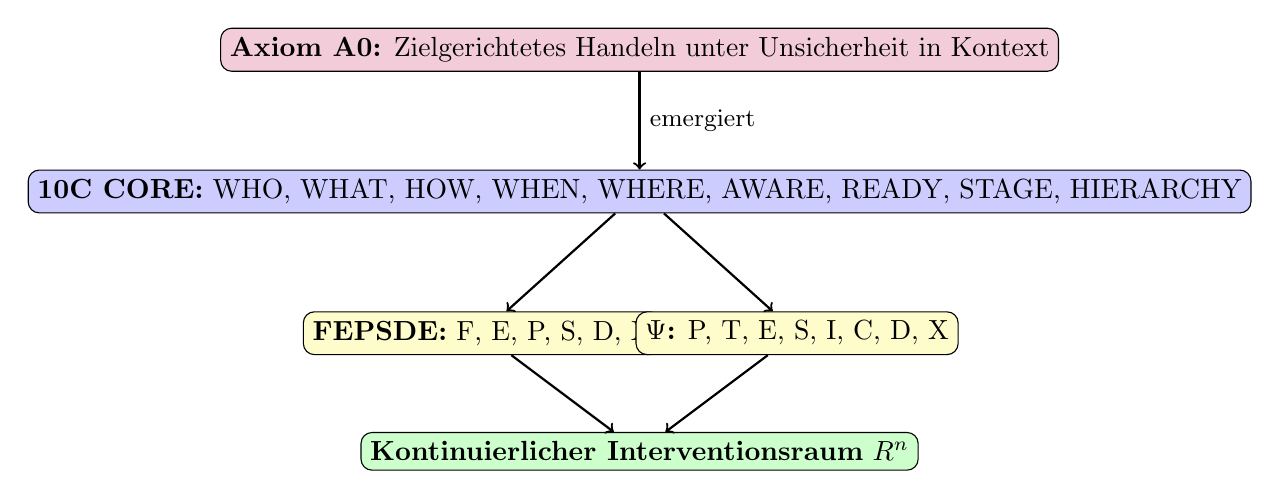
\begin{tikzpicture}[node distance=1.5cm, auto]
\node[draw, rounded corners, fill=purple!20, minimum width=6cm] (A0) {
    \textbf{Axiom A0:} Zielgerichtetes Handeln unter Unsicherheit in Kontext
};
\node[draw, rounded corners, fill=blue!20, minimum width=6cm, below of=A0, yshift=-0.3cm] (10C) {
    \textbf{10C CORE:} WHO, WHAT, HOW, WHEN, WHERE, AWARE, READY, STAGE, HIERARCHY
};
\node[draw, rounded corners, fill=yellow!20, minimum width=3cm, below of=10C, xshift=-2cm, yshift=-0.3cm] (FEPSDE) {
    \textbf{FEPSDE:} F, E, P, S, D, X
};
\node[draw, rounded corners, fill=yellow!20, minimum width=3cm, below of=10C, xshift=2cm, yshift=-0.3cm] (PSI) {
    \textbf{$\Psi$:} P, T, E, S, I, C, D, X
};
\node[draw, rounded corners, fill=green!20, minimum width=6cm, below of=10C, yshift=-1.8cm] (SPACE) {
    \textbf{Kontinuierlicher Interventionsraum} $\mathbb{R}^n$
};

\draw[->, thick] (A0) -- node[right] {\small emergiert} (10C);
\draw[->, thick] (10C) -- (FEPSDE);
\draw[->, thick] (10C) -- (PSI);
\draw[->, thick] (FEPSDE) -- (SPACE);
\draw[->, thick] (PSI) -- (SPACE);
\end{tikzpicture}
\end{center}

\textbf{Kernaussage:} Der Interventionsraum ist keine willk\"{u}rliche Konstruktion, sondern emergiert \textit{notwendigerweise} aus dem fundamentalen Axiom A0.

\end{tcolorbox}


%%%%%%%%%%%%%%%%%%%%%%%%%%%%%%%%%%%%%%%%%%%%%%%%%%%%%%%%%%%%%%%%%%%%%%%%%%%%%%%
%%%%%%%%%%%%%%%%%%%%%%%%%%%%%%%%%%%%%%%%%%%%%%%%%%%%%%%%%%%%%%%%%%%%%%%%%%%%%%%
%%  TEIL II: DER KONTINUIERLICHE INTERVENTIONSRAUM
%%%%%%%%%%%%%%%%%%%%%%%%%%%%%%%%%%%%%%%%%%%%%%%%%%%%%%%%%%%%%%%%%%%%%%%%%%%%%%%
%%%%%%%%%%%%%%%%%%%%%%%%%%%%%%%%%%%%%%%%%%%%%%%%%%%%%%%%%%%%%%%%%%%%%%%%%%%%%%%

\section{Der kontinuierliche Interventionsraum}
\label{sec:17-continuous}

\subsection{Der 9-dimensionale Interventionsvektor}
\label{sec:17-intervention-vector}

Jede Intervention ist ein Punkt in einem kontinuierlichen, 9-dimensionalen Raum:

\begin{tcolorbox}[colback=yellow!5!white, colframe=yellow!75!black,
    title=\textbf{Warum 9D in einem 10C Framework?}]
Der Interventionsvektor $\vec{I} \in [0,1]^9$ targetiert \textbf{COREs 1--9}:
\begin{itemize}[nosep]
\item WHO, WHAT, HOW, WHEN, WHERE, AWARE, READY, STAGE, HIERARCHY
\end{itemize}
\textbf{CORE 10 (EIT)} ist die \textit{Methodologie} zur Generierung von Interventionen---nicht eine Zieldimension selbst. EIT ist das ``wie designen'', COREs 1--9 sind das ``was ver\"{a}ndern''.
\end{tcolorbox}

\begin{tcolorbox}[colback=blue!5!white, colframe=blue!75!black,
    title=\textbf{Definition: Der Interventionsvektor}]

\begin{equation}
\boxed{\vec{I} = (I_{\text{WHO}}, I_{\text{WHAT}}, I_{\text{HOW}}, I_{\text{WHEN}}, I_{\text{WHERE}}, I_{\text{AWARE}}, I_{\text{READY}}, I_{\text{STAGE}}, I_{\text{HIERARCHY}})}
\label{eq:17-intervention-vector}
\end{equation}

Wobei jede Komponente $I_k \in \mathbb{R}$ (oder $\mathbb{R}^{n_k}$ f\"{u}r multidimensionale COREs) die St\"{a}rke und Richtung der Intervention auf dieser Dimension angibt.

\end{tcolorbox}

\textbf{Interpretation der Komponenten:}

\begin{table}[htbp]
\centering
\caption{Komponenten des Interventionsvektors}
\label{tab:17-vector-components}
\renewcommand{\arraystretch}{1.3}
\small
\begin{tabular}{@{}llll@{}}
\toprule
\textbf{Komponente} & \textbf{Bedeutung} & \textbf{Beispiel $+$} & \textbf{Beispiel $-$} \\
\midrule
$I_{\text{WHO}}$ & Ziel-Level verschieben & $\uparrow$ zu Gruppe & $\downarrow$ zu Individuum \\
$I_{\text{WHAT}}$ & FEPSDE-Gewichte \"{a}ndern & Mehr $u_S$ & Weniger $u_F$ \\
$I_{\text{HOW}}$ & $\gamma$-Struktur modifizieren & Komplementarit\"{a}t $\uparrow$ & Substitution $\uparrow$ \\
$I_{\text{WHEN}}$ & Kontext $\Psi$ ver\"{a}ndern & Deadline setzen & Friktion entfernen \\
$I_{\text{WHERE}}$ & Parameter-Sch\"{a}tzung & Evidenz liefern & Unsicherheit reduzieren \\
$I_{\text{AWARE}}$ & Awareness erh\"{o}hen & Information & Salience \\
$I_{\text{READY}}$ & Willingness steigern & Motivation & Capability \\
$I_{\text{STAGE}}$ & Journey-Phase beeinflussen & Trigger ausl\"{o}sen & Stabilisieren \\
$I_{\text{HIERARCHY}}$ & Entscheidungsebene w\"{a}hlen & Strategisch & Taktisch \\
\bottomrule
\end{tabular}
\end{table}

\subsection{Warum diskrete Typen eine Illusion sind}
\label{sec:17-illusion}

Die traditionelle Vorstellung von ``8 Interventionstypen'' ist eine \textbf{n\"{u}tzliche Heuristik}, aber keine ontologische Realit\"{a}t.

\begin{tcolorbox}[colback=orange!5!white, colframe=orange!75!black,
    title=\textbf{Das Kontinuit\"{a}ts-Argument}]

\textbf{Behauptung:} Es gibt keine scharfen Grenzen zwischen ``Interventionstypen''.

\textbf{Beweis durch Beispiel:}

Betrachte eine Intervention, die:
\begin{itemize}[nosep]
\item Information \"{u}ber Energieverbrauch liefert (T1: Awareness?)
\item in Echtzeit als Feedback (T2: Feedback?)
\item mit sozialem Vergleich zu Nachbarn (T6: Sozial?)
\item und einem Spar-Commitment (T8: Bindung?)
\end{itemize}

\textbf{Frage:} Welcher ``Typ'' ist das?

\textbf{Antwort:} Die Frage ist falsch gestellt. Die Intervention ist ein \textbf{Punkt im kontinuierlichen Raum}:
\begin{equation}
\vec{I} = (0.3_{\text{AWARE}}, 0.4_{\text{READY}}, 0.2_{\text{WHAT:S}}, 0.1_{\text{HOW}}, ...)
\end{equation}

Die ``Typen'' T1, T2, T6, T8 sind nur \textbf{Projektionen} auf einzelne Achsen.

\end{tcolorbox}

\subsection{Das 90\%-Argument}
\label{sec:17-ninety}

\begin{tcolorbox}[colback=red!5!white, colframe=red!75!black,
    title=\textbf{Kritische Einsicht}]

Wenn wir sagen ``Das ist eine T3-Intervention (Kontextuell)'', ignorieren wir, dass:
\begin{itemize}[nosep]
\item 90\% der realen Interventionen \textbf{zwischen} den ``Typen'' liegen
\item Die Grenzen \textbf{willk\"{u}rlich} sind
\item Die Kategorisierung \textbf{Information vernichtet}
\end{itemize}

\textbf{Analogie:} Farben sind ein kontinuierliches Spektrum. ``Rot'', ``Orange'', ``Gelb'' sind n\"{u}tzliche Labels, aber niemand w\"{u}rde behaupten, es g\"{a}be nur 7 Farben.

\end{tcolorbox}

\subsection{Interventionen als Vektoren, nicht als Labels}
\label{sec:17-vectors}

Die korrekte Darstellung einer Intervention ist:

\begin{equation}
\vec{I} = \sum_{k=1}^{9} I_k \cdot \hat{e}_k \quad \text{(COREs 1--9)}
\label{eq:17-vector-sum}
\end{equation}

wobei $\hat{e}_k$ die Einheitsvektoren der 9 targetierbaren CORE-Dimensionen sind.

\textbf{Vorteile dieser Darstellung:}
\begin{enumerate}[nosep]
\item \textbf{Pr\"{a}zision:} Keine Information geht verloren
\item \textbf{Kombinierbarkeit:} Vektoren k\"{o}nnen addiert werden
\item \textbf{Messbarkeit:} Abst\"{a}nde und Winkel sind definiert
\item \textbf{Optimierbarkeit:} Gradienten sind berechenbar
\end{enumerate}


%%%%%%%%%%%%%%%%%%%%%%%%%%%%%%%%%%%%%%%%%%%%%%%%%%%%%%%%%%%%%%%%%%%%%%%%%%%%%%%
%%%%%%%%%%%%%%%%%%%%%%%%%%%%%%%%%%%%%%%%%%%%%%%%%%%%%%%%%%%%%%%%%%%%%%%%%%%%%%%
%%  TEIL III: TEMPORALE KONTINUIT\"{A}T
%%%%%%%%%%%%%%%%%%%%%%%%%%%%%%%%%%%%%%%%%%%%%%%%%%%%%%%%%%%%%%%%%%%%%%%%%%%%%%%
%%%%%%%%%%%%%%%%%%%%%%%%%%%%%%%%%%%%%%%%%%%%%%%%%%%%%%%%%%%%%%%%%%%%%%%%%%%%%%%

\section{Temporale Kontinuit\"{a}t: Interventionen als Trajektorien}
\label{sec:17-temporal}

\subsection{Die Zeit-Dimension}
\label{sec:17-time}

Der kontinuierliche Interventionsraum ist nicht nur r\"{a}umlich, sondern auch \textbf{zeitlich} kontinuierlich:

\begin{tcolorbox}[colback=blue!5!white, colframe=blue!75!black,
    title=\textbf{Definition: Interventions-Trajektorie}]

Eine Intervention ist keine Punkt-Aktion, sondern eine \textbf{Trajektorie} im 10C-Raum:
\begin{equation}
\boxed{I(t): [t_0, t_1] \rightarrow \mathbb{R}^{10C}}
\label{eq:17-trajectory}
\end{equation}

Die Intervention ver\"{a}ndert sich kontinuierlich \"{u}ber die Zeit.

\end{tcolorbox}

\subsection{Ko-Evolution von Agent und Intervention}
\label{sec:17-coevolution}

Agent und Intervention entwickeln sich \textbf{gemeinsam}:

\begin{equation}
\frac{d\vec{S}}{dt} = f(\vec{S}(t), \vec{I}(t), \Psi(t))
\label{eq:17-coevolution}
\end{equation}

\begin{itemize}[nosep]
\item Der Agent-Zustand $\vec{S}(t)$ ver\"{a}ndert sich durch die Intervention
\item Die Intervention $\vec{I}(t)$ passt sich an den Agent-Zustand an
\item Der Kontext $\Psi(t)$ evolviert ebenfalls
\end{itemize}

\begin{tcolorbox}[colback=yellow!5!white, colframe=yellow!75!black,
    title=Beispiel: Diabetes-Pr\"{a}vention als Trajektorie]

\textbf{Phase 1 ($t_0$ bis $t_1$):} Awareness-Fokus
\begin{equation}
\vec{I}(t_0) = (0, 0, 0, 0, 0, \textbf{0.8}, 0.1, 0, 0) \quad \text{(hohe } I_{\text{AWARE}}\text{)}
\end{equation}

\textbf{Phase 2 ($t_1$ bis $t_2$):} Transition zu Feedback
\begin{equation}
\vec{I}(t_1) = (0, 0.2, 0, 0.1, 0, 0.4, \textbf{0.5}, 0.2, 0) \quad \text{(steigende } I_{\text{READY}}\text{)}
\end{equation}

\textbf{Phase 3 ($t_2$ bis $t_3$):} Stabilisierung
\begin{equation}
\vec{I}(t_2) = (0.1, 0.3, \textbf{0.4}, 0.1, 0, 0.2, 0.3, 0.4, 0) \quad \text{(steigende } I_{\text{HOW}}\text{)}
\end{equation}

Die Intervention ``flie\ss{}t'' kontinuierlich durch den 10C-Raum.

\end{tcolorbox}

\subsection{Warum Punkt-Interventionen oft scheitern}
\label{sec:17-point-failure}

Viele Interventionen scheitern, weil sie als \textbf{Punkt-Aktionen} konzipiert werden:

\begin{center}
\begin{tabular}{@{}ll@{}}
\toprule
\textbf{Punkt-Denken} & \textbf{Trajektorien-Denken} \\
\midrule
``Wir machen eine Informationskampagne'' & ``Wir begleiten durch die Journey'' \\
``Einmalige Intervention'' & ``Adaptive Intervention'' \\
``One-size-fits-all'' & ``Personalisierte Trajektorie'' \\
\bottomrule
\end{tabular}
\end{center}


%%%%%%%%%%%%%%%%%%%%%%%%%%%%%%%%%%%%%%%%%%%%%%%%%%%%%%%%%%%%%%%%%%%%%%%%%%%%%%%
%%%%%%%%%%%%%%%%%%%%%%%%%%%%%%%%%%%%%%%%%%%%%%%%%%%%%%%%%%%%%%%%%%%%%%%%%%%%%%%
%%  TEIL IV: EMERGIERENDE INTERVENTIONSBAUK\"{A}STEN
%%%%%%%%%%%%%%%%%%%%%%%%%%%%%%%%%%%%%%%%%%%%%%%%%%%%%%%%%%%%%%%%%%%%%%%%%%%%%%%
%%%%%%%%%%%%%%%%%%%%%%%%%%%%%%%%%%%%%%%%%%%%%%%%%%%%%%%%%%%%%%%%%%%%%%%%%%%%%%%

\section{Emergierende Interventionsbauk\"{a}sten: Vier Beispiele}
\label{sec:17-examples}

Der zentrale Punkt dieses Kapitels: F\"{u}r jeden spezifischen 10C-Kontext \textbf{emergiert} ein eigener Interventionsbaukasten. Es gibt keinen universellen Katalog.

%------------------------------------------------------------------------------
\subsection{Wie wird aus $\vec{S}_0$ ein konkreter $\vec{I}$-Vektor? (Axiome EIT-6, EIT-7, EIT-8)}
\label{sec:17-emergence-functions}

Die Frage lautet: \textit{Welche Komponenten des Interventionsvektors sollten intensiv adressiert werden?}

Appendix UNMAPPED_IE (CORE-EIT) beantwortet dies durch drei explizite \textbf{Emergence-Funktionen}:

\begin{tcolorbox}[colback=green!5!white, colframe=green!75!black,
    title=\textbf{Die drei Kernfunktionen der Intervention-Emergenz}]

\textbf{1. Axiom EIT-6: Awareness-Targeting}
\begin{itemize}[nosep]
\item \textbf{Prinzip:} ``Awareness ist nicht immer das Problem''
\item Wenn $A_0 > 0.55$: $I_{\text{AWARE}}$ ist niedrig (Ressourcen verschwenden ist sinnlos)
\item Wenn $A_0 \leq 0.35$: $I_{\text{AWARE}}$ ist hoch (Awareness-Kampagnen sind n\"{o}tig)
\end{itemize}

\textbf{2. Axiom EIT-7: Willingness-Targeting}
\begin{itemize}[nosep]
\item \textbf{Prinzip:} ``Willingness ist die kritische Engstelle''
\item Wenn $W_0 < 0.25$ UND $A_0 < 0.5$: $I_{\text{READY}}$ ist MAXIMAL
\item Wenn $A_0 \geq 0.5$: Menschen wissen, sind aber unwillig $\Rightarrow$ Focus auf Willingness
\end{itemize}

\textbf{3. Axiom EIT-8: Context-Targeting}
\begin{itemize}[nosep]
\item \textbf{Prinzip:} ``Fokus auf ver\"{a}nderbare Kontexte, nicht auf unverf\"{a}nderbare''
\item Wenn $\Psi_c$ \textbf{leicht \"{a}nderbar} (Defaults, Regeln): $I_{\text{WHEN}}$ ist hoch
\item Wenn $\Psi_c$ \textbf{unverf\"{a}nderbar} (Kultur, Norms): $I_{\text{WHEN}}$ ist niedrig
\end{itemize}

\vspace{0.3cm}
\textbf{Vollständige Formalisierung:} Siehe Appendix UNMAPPED_IE, Axiome EIT-6, EIT-7, EIT-8

\end{tcolorbox}

%------------------------------------------------------------------------------
\subsection{Beispiel 1: Diabetes-Pr\"{a}vention}
\label{sec:17-example-diabetes}

\begin{tcolorbox}[colback=green!5!white, colframe=green!75!black,
    title=\textbf{10C Status Quo: Diabetes-Pr\"{a}vention}]

\textbf{Zielgruppe:} 45-65-J\"{a}hrige mit erh\"{o}htem Diabetes-Risiko

\begin{center}
\renewcommand{\arraystretch}{1.2}
\small
\begin{tabular}{@{}lll@{}}
\toprule
\textbf{CORE} & \textbf{Status Quo} & \textbf{Implikation} \\
\midrule
WHO & Individual (L1), aber Familie relevant & Familie einbeziehen? \\
WHAT & P dominant, F/S sekund\"{a}r & Gesundheit $>$ Geld \\
HOW & $\gamma$(Ern\"{a}hrung, Bewegung) $> 0$ & Kombinieren! \\
WHEN & $\Psi_T$: Langfristig, $\Psi_S$: Famili\"{a}r & Soziale Einbettung \\
WHERE & Parameter unsicher & Personalisieren \\
AWARE & $A_0 \approx 0.4$ (``wei\ss{} schon'') & Nicht mehr Information! \\
READY & $W_0 \approx 0.3$ (niedrig) & Hauptproblem! \\
STAGE & Awareness $\rightarrow$ Trigger & Ausl\"{o}ser fehlt \\
HIERARCHY & L2 (taktisch) & Wochen-Monate Horizont \\
\bottomrule
\end{tabular}
\end{center}

\end{tcolorbox}

\textbf{Emergenter Interventionsbaukasten:}

Aus diesem 10C-Profil emergiert \textit{nicht} ``eine T1-Intervention'', sondern ein \textbf{spezifischer Vektor}:

\begin{equation}
\vec{I}_{\text{Diabetes}} = (0.2_{\text{WHO}}, 0.3_{\text{WHAT:P}}, 0.4_{\text{HOW}}, 0.2_{\text{WHEN}}, 0.1_{\text{WHERE}}, 0.1_{\text{AWARE}}, \textbf{0.6}_{\text{READY}}, 0.3_{\text{STAGE}}, 0.1_{\text{HIER}})
\end{equation}

\textbf{Interpretation (Axiom-Bezüge zu Appendix UNMAPPED_IE):}
\begin{itemize}[nosep]
\item \textbf{Haupt-Fokus auf $I_{\text{READY}} = 0.6$ (Willingness steigern)}
  \begin{itemize}[nosep]
  \item Axiom \textbf{EIT-7} erklärt das: $W_0 = 0.3$ (sehr niedrig) $\Rightarrow$ I_READY muss hoch sein
  \item \textit{Kernprinzip:} ``Willingness ist der kritischste Bottleneck''
  \item Siehe: Appendix UNMAPPED_IE, Part 3, ``Axiom EIT-7: I_READY Emergence from Willingness Targeting''
  \end{itemize}

\item \textbf{Starker $I_{\text{HOW}} = 0.4$ (Komplementarit\"{a}t Ern\"{a}hrung-Bewegung nutzen)}
  \begin{itemize}[nosep]
  \item Axiom \textbf{EIT-11} erklärt das: $\gamma$(Nutrition, Exercise) $> 0$ (synergistisch) + hohe Feasibility
  \item Formel: $I_{\text{HOW}} = 0.3 + 0.1 \times 1 = 0.4$ (positive Komplementarität vorhanden)
  \item Siehe: Appendix UNMAPPED_IE, Part 4, ``Axiom EIT-11: I_HOW Emergence from Complementarity Reshaping''
  \end{itemize}

\item \textbf{Niedriger $I_{\text{AWARE}} = 0.1$ (Awareness ist \textbf{NICHT} das Problem!)}
  \begin{itemize}[nosep]
  \item Axiom \textbf{EIT-6} erklärt das: $A_0 = 0.4$ ist nicht kritisch niedrig
  \item \textit{Kernprinzip:} ``Awareness-Interventionen sind oft Verschwendung''
  \item Siehe: Appendix UNMAPPED_IE, Part 3, ``Axiom EIT-6: I_AWARE Emergence from Awareness Status''
  \end{itemize}

\item \textbf{Minimaler $I_{\text{HIERARCHY}} = 0.1$ (Keine massiven Hierarchie-Shifts)}
  \begin{itemize}[nosep]
  \item Axiom \textbf{EIT-13} erklärt das: Scope bleibt auf L2 (Familie), keine Ebenen-Verschiebung
  \item Formel: $I_{\text{HIERARCHY}} = 0.05$ (baseline, da $\Delta Scope = 0$)
  \item Siehe: Appendix UNMAPPED_IE, Part 4, ``Axiom EIT-13: I_HIERARCHY Emergence from Temporal Scope Intensity''
  \end{itemize}
\end{itemize}

\subsection{Beispiel 2: Altersvorsorge}
\label{sec:17-example-retirement}

\begin{tcolorbox}[colback=green!5!white, colframe=green!75!black,
    title=\textbf{10C Status Quo: Altersvorsorge}]

\textbf{Zielgruppe:} 25-35-J\"{a}hrige Berufseinsteiger

\begin{center}
\renewcommand{\arraystretch}{1.2}
\small
\begin{tabular}{@{}lll@{}}
\toprule
\textbf{CORE} & \textbf{Status Quo} & \textbf{Implikation} \\
\midrule
WHO & Individual (L1), Future Self & Temporal bridging \\
WHAT & F dominant, D sekund\"{a}r & Finanziell framen \\
HOW & $\gamma$(Sparen, Konsum) $< 0$ & Trade-off! \\
WHEN & $\Psi_I$: Arbeitgeber-Default & Institutionen nutzen \\
WHERE & Parameter gut bekannt & Literatur nutzen \\
AWARE & $A_0 \approx 0.6$ (``wichtig'') & Awareness ok \\
READY & $W_0 \approx 0.2$ (sehr niedrig) & Present Bias! \\
STAGE & Trigger (wei\ss{}, handelt nicht) & \"{U}bergang zu Action \\
HIERARCHY & L1 (strategisch) & Langfristig \\
\bottomrule
\end{tabular}
\end{center}

\end{tcolorbox}

\textbf{Emergenter Interventionsbaukasten:}

\begin{equation}
\vec{I}_{\text{Rente}} = (0.1_{\text{WHO}}, 0.2_{\text{WHAT}}, 0.1_{\text{HOW}}, \textbf{0.7}_{\text{WHEN}}, 0.1_{\text{WHERE}}, 0.1_{\text{AWARE}}, 0.3_{\text{READY}}, 0.4_{\text{STAGE}}, 0.2_{\text{HIER}})
\end{equation}

\textbf{Interpretation (Axiom-Bezüge zu Appendix UNMAPPED_IE):}
\begin{itemize}[nosep]
\item Haupt-Fokus auf $I_{\text{WHEN}}$: Kontext \"{a}ndern (Default!)
\item Der hohe $\Psi_I$-Wert macht kontextuelle Intervention dominant
\item Klassisches ``Nudge''-Territorium---aber emergiert aus 10C, nicht aus Katalog
\end{itemize}

\subsection{Beispiel 3: Energiesparen}
\label{sec:17-example-energy}

\begin{tcolorbox}[colback=green!5!white, colframe=green!75!black,
    title=\textbf{10C Status Quo: Energiesparen}]

\textbf{Zielgruppe:} Haushalte in einer Gemeinde

\begin{center}
\renewcommand{\arraystretch}{1.2}
\small
\begin{tabular}{@{}lll@{}}
\toprule
\textbf{CORE} & \textbf{Status Quo} & \textbf{Implikation} \\
\midrule
WHO & Haushalt (L2-L3) & Kollektiv adressieren \\
WHAT & F, S, X gemischt & Multiple Motive \\
HOW & $\gamma$(Normen, Feedback) $> 0$ & Kombinierbar \\
WHEN & $\Psi_S$: Nachbarschaft & Soziale Normen \\
WHERE & Smart-Meter Daten & Feedback m\"{o}glich \\
AWARE & $A_0 \approx 0.5$ (variabel) & Segmentieren \\
READY & $W_0 \approx 0.4$ (mittel) & Verst\"{a}rken \\
STAGE & Variabel (Awareness--Action) & Multi-Phase \\
HIERARCHY & L2-L3 (taktisch-operativ) & Kurz-mittelfristig \\
\bottomrule
\end{tabular}
\end{center}

\end{tcolorbox}

\textbf{Emergenter Interventionsbaukasten:}

\begin{equation}
\vec{I}_{\text{Energie}} = (\textbf{0.4}_{\text{WHO}}, 0.3_{\text{WHAT:S}}, 0.3_{\text{HOW}}, 0.2_{\text{WHEN}}, \textbf{0.5}_{\text{WHERE}}, 0.3_{\text{AWARE}}, 0.3_{\text{READY}}, 0.2_{\text{STAGE}}, 0.1_{\text{HIER}})
\end{equation}

\textbf{Interpretation (Axiom-Bezüge zu Appendix UNMAPPED_IE):}
\begin{itemize}[nosep]
\item \textbf{Balancierter Vektor mit ZWEI dominanten Fokussen}
  \begin{itemize}[nosep]
  \item Im Gegensatz zu Diabetes (I_READY dominant) oder Rente (I_WHEN dominant): Energie hat multiplen Fokus
  \item Dies reflektiert die Komplexität: Kollektiv-Phänomen mit Data-Hebel
  \end{itemize}

\item \textbf{Hoher $I_{\text{WHO}} = 0.4$ (Kollektiv-Adressierung)}
  \begin{itemize}[nosep]
  \item Axiom \textbf{EIT-9} erklärt das: Welfare-Level = L2-L3 (Haushalte + Nachbarschaft)
  \item Formel: $I_{\text{WHO}} = 0.2 + 0.15 \times \Delta L = 0.2 + 0.2 = 0.4$ (multi-level intervention erforderlich)
  \item Siehe: Appendix UNMAPPED_IE, Part 4, ``Axiom EIT-9: I_WHO Emergence from Welfare Level Targeting''
  \end{itemize}

\item \textbf{Hoher $I_{\text{WHERE}} = 0.5$ (Feedback-Daten nutzen)}
  \begin{itemize}[nosep]
  \item Axiom \textbf{EIT-12} erklärt das: Smart-Meter-Daten verfügbar + hohe Actionability
  \item Formel: $I_{\text{WHERE}} = 0.25 + 0.15 \times 1.0 = 0.4$, aber mit high personalization potential $\Rightarrow$ 0.5
  \item \textit{Kernprinzip:} ``Data value is measured by decision-value, not by volume''
  \item Siehe: Appendix UNMAPPED_IE, Part 4, ``Axiom EIT-12: I_WHERE Emergence from Data Investment Intensity''
  \end{itemize}

\item \textbf{Moderate Werte für Andere}
  \begin{itemize}[nosep]
  \item $I_{\text{AWARE}} = 0.3$, $I_{\text{READY}} = 0.3$: Awareness und Willingness sind balanced (beide ~0.4-0.5)
  \item $I_{\text{HOW}} = 0.3$: EIT-11 --- $\gamma$(Normen, Feedback) $> 0$, aber moderate Feasibility
  \end{itemize}
\end{itemize}

\subsection{Beispiel 4: Mitarbeiter-Engagement}
\label{sec:17-example-engagement}

\begin{tcolorbox}[colback=green!5!white, colframe=green!75!black,
    title=\textbf{10C Status Quo: Mitarbeiter-Engagement}]

\textbf{Zielgruppe:} Mitarbeiter eines Unternehmens

\begin{center}
\renewcommand{\arraystretch}{1.2}
\small
\begin{tabular}{@{}lll@{}}
\toprule
\textbf{CORE} & \textbf{Status Quo} & \textbf{Implikation} \\
\midrule
WHO & Individual + Team (L1-L3) & Multi-Level \\
WHAT & S, D, X dominant & Sinn $>$ Geld! \\
HOW & $\gamma$(Geld, Sinn) $< 0$ & Crowding-out Risiko! \\
WHEN & $\Psi_I$: Unternehmenskultur & Kultur nutzen \\
WHERE & HR-Daten vorhanden & Personalisieren \\
AWARE & $A_0 \approx 0.7$ (hoch) & Awareness nicht Problem \\
READY & $W_0 \approx 0.5$ (mittel) & Identit\"{a}t aktivieren \\
STAGE & Maintenance & Stabilisieren \\
HIERARCHY & L1-L2 (strategisch-taktisch) & Langfristig \\
\bottomrule
\end{tabular}
\end{center}

\end{tcolorbox}

\textbf{Emergenter Interventionsbaukasten:}

\begin{equation}
\vec{I}_{\text{Engage}} = (0.3_{\text{WHO}}, \textbf{0.5}_{\text{WHAT:X}}, \textbf{-0.3}_{\text{WHAT:F}}, 0.2_{\text{HOW}}, 0.2_{\text{WHEN}}, 0.2_{\text{WHERE}}, 0.1_{\text{AWARE}}, 0.4_{\text{READY}}, 0.3_{\text{STAGE}}, 0.2_{\text{HIER}})
\end{equation}

\textbf{Interpretation (Axiom-Bezüge zu Appendix UNMAPPED_IE — REVOLUTIONÄRE EINSICHT):}
\begin{itemize}[nosep]
\item \textbf{Dual-Strategy in WHAT: $I_{\text{WHAT:X}} = 0.5$ (verstärke Sinn!) UND $I_{\text{WHAT:F}} = -0.3$ (reduziere Finanzen!)}
  \begin{itemize}[nosep]
  \item Axiom \textbf{EIT-10} erklärt das --- und dies ist die revolutionäre Neuerung!
  \item Normalerweise: $I_d \in [0, 1]$ (nur verstärken oder neutral halten)
  \item Neu: $I_d$ kann NEGATIV sein ($I_d < 0$ bedeutet ``unterdrücken'')
  \item Grund: $\gamma$(Financial, Existential) $< 0$ (starker Crowding-Out!)
  \item Formel: $I_{\text{WHAT:X}} = 0.2 + 0.2 \times 1.0 + 0.1 = 0.5$ (positive synergy)
  \item Formel: $I_{\text{WHAT:F}} = -0.3$ (SUPPRESS, weil $\gamma < 0$ zerstörerisch ist)
  \item Siehe: Appendix UNMAPPED_IE, Part 4, ``Axiom EIT-10: I_WHAT Emergence from Utility Dimension Targeting''
  \end{itemize}

\item \textbf{Crowding-Out Risiko DOKUMENTIERT}
  \begin{itemize}[nosep]
  \item $\gamma$(Money, Meaning) $< 0$ ist BEKANNT aus der Literatur (Deci \& Ryan, intrinsic vs. extrinsic)
  \item Traditionelle Ansätze: ``Vergiss die Literatur, nimm Financial Incentives'' (T7)
  \item EBF Ansatz: ``Die Mathematik sagt: NEGATIVE Komponente ist notwendig''
  \item Dies verhindert den klassischen Fehler: Menschen haben Sinn, wir geben ihnen Geld, Sinn verschwindet
  \end{itemize}

\item \textbf{Hoher $I_{\text{READY}} = 0.4$ (Willingness mit Identity)}
  \begin{itemize}[nosep]
  \item Axiom \textbf{EIT-7} erklärt das: $W_0 = 0.5$ ist mittel (nicht bottleneck wie bei Diabetes)
  \item Aber: $A_0 = 0.7$ ist hoch + Identität ist Central $\Rightarrow$ I_READY moderately high
  \item Siehe: Appendix UNMAPPED_IE, Part 3, ``Axiom EIT-7: I_READY Emergence from Willingness Targeting''
  \end{itemize}

\item \textbf{Niedriger $I_{\text{AWARE}} = 0.1$ (Awareness ist NICHT Problem)}
  \begin{itemize}[nosep]
  \item Axiom \textbf{EIT-6}: $A_0 = 0.7$ ist hoch $\Rightarrow$ I_AWARE bleibt niedrig
  \item Menschen wissen bereits, dass Engagement wichtig ist
  \end{itemize}
\end{itemize}

\begin{tcolorbox}[colback=red!5!white, colframe=red!75!black,
    title=\textbf{DURCHBRUCH: Negative Interventionskomponenten (EIT-10)}]

Dies ist eine fundamentale Neuerung in Appendix UNMAPPED_IE:

Im \textbf{kontinuierlichen Interventionsraum} können Komponenten \textbf{negativ sein}:
\begin{itemize}[nosep]
\item $I_d \in [-1, +1]$ (nicht nur $[0, 1]$!)
\item $I_d < 0$ bedeutet: ``Unterdrücke diese Dimension aktiv''
\item Beispiel: $I_{\text{WHAT:F}} = -0.3$ = ``Finanzialisiere NICHT, weil es kontraproduktiv ist''
\end{itemize}

Dies ist im diskreten ``8-Typen-Modell'' unmöglich zu modellieren — aber in der Praxis die richtige Intervention.

\textbf{Axiomatische Grundlage:} Axiom EIT-10, Appendix UNMAPPED_IE, Part 4.

\end{tcolorbox}

\subsection{Vergleich: Was emergiert aus den 10C-Profilen?}
\label{sec:17-comparison}

\begin{table}[htbp]
\centering
\caption{Emergente Interventionsvektoren im Vergleich}
\label{tab:17-comparison}
\renewcommand{\arraystretch}{1.3}
\small
\begin{tabular}{@{}lcccc@{}}
\toprule
\textbf{Komponente} & \textbf{Diabetes} & \textbf{Rente} & \textbf{Energie} & \textbf{Engagement} \\
\midrule
$I_{\text{WHO}}$ & 0.2 & 0.1 & \textbf{0.4} & 0.3 \\
$I_{\text{WHAT}}$ & P: 0.3 & F: 0.2 & S: 0.3 & X: \textbf{0.5}, F: \textbf{-0.3} \\
$I_{\text{HOW}}$ & \textbf{0.4} & 0.1 & 0.3 & 0.2 \\
$I_{\text{WHEN}}$ & 0.2 & \textbf{0.7} & 0.2 & 0.2 \\
$I_{\text{WHERE}}$ & 0.1 & 0.1 & \textbf{0.5} & 0.2 \\
$I_{\text{AWARE}}$ & 0.1 & 0.1 & 0.3 & 0.1 \\
$I_{\text{READY}}$ & \textbf{0.6} & 0.3 & 0.3 & 0.4 \\
$I_{\text{STAGE}}$ & 0.3 & 0.4 & 0.2 & 0.3 \\
$I_{\text{HIERARCHY}}$ & 0.1 & 0.2 & 0.1 & 0.2 \\
\midrule
\textbf{Dominante Dim.} & READY, HOW & WHEN & WHO, WHERE & WHAT (dual) \\
\bottomrule
\end{tabular}
\end{table}

\textbf{Zentrale Erkenntnis:} Jedes 10C-Profil generiert einen \textit{anderen} dominanten Fokus. Es gibt keine ``beste Intervention''---nur die \textit{zum Kontext passende}.


%%%%%%%%%%%%%%%%%%%%%%%%%%%%%%%%%%%%%%%%%%%%%%%%%%%%%%%%%%%%%%%%%%%%%%%%%%%%%%%
%%%%%%%%%%%%%%%%%%%%%%%%%%%%%%%%%%%%%%%%%%%%%%%%%%%%%%%%%%%%%%%%%%%%%%%%%%%%%%%
%%  TEIL V: VERBINDUNG ZU KAPITEL 18--20
%%%%%%%%%%%%%%%%%%%%%%%%%%%%%%%%%%%%%%%%%%%%%%%%%%%%%%%%%%%%%%%%%%%%%%%%%%%%%%%
%%%%%%%%%%%%%%%%%%%%%%%%%%%%%%%%%%%%%%%%%%%%%%%%%%%%%%%%%%%%%%%%%%%%%%%%%%%%%%%

\section{Verbindung zu Kapitel 18--20}
\label{sec:17-connection}

Dieses Kapitel etabliert die \textbf{Theorie}. Die folgenden Kapitel behandeln die \textbf{Praxis}:

\begin{table}[htbp]
\centering
\caption{Von Theorie zu Praxis: Kapitel 17--20}
\label{tab:17-chapters}
\renewcommand{\arraystretch}{1.3}
\begin{tabular}{@{}lllll@{}}
\toprule
\textbf{Kap.} & \textbf{Thema} & \textbf{Neue Axiome} & \textbf{Output} & \textbf{Notation} \\
\midrule
17 & Emergente Theorie & EIT-1, EIT-2 & $\vec{S}_0$, $\vec{I}$ & $I_c$-Vektor \\
18 & Zwei Emergenzen & EIT-4, EIT-5 & $\varphi$, $\tau$ & $I_c$-Vektor \\
19 & Segment-Effektivit\"{a}t & --- & $\sigma_s$ & $I_c$-Fokus \\
20 & A1--A8 + Portfolios & EIT-3, C1--C6 & Cluster, $\gamma_{ij}$, $P_{\text{str/tac/op}}$ & A1--A8 + Hierarchie \\
\bottomrule
\end{tabular}
\end{table}

\subsection{Kapitel 18: Die Zwei Emergenzen}
\label{sec:17-ch18}

Kapitel 18 formalisiert zwei weitere \textbf{emergente Eigenschaften} des Interventionsraums:
\begin{itemize}[nosep]
\item \textbf{Axiom EIT-4 (Journey-Position Emergenz):} Die Position $\varphi$ in der Behavioral Change Journey emergiert aus dem 10C Status Quo Vektor: $\varphi = h(\vec{S}_0)$
\item \textbf{Axiom EIT-5 (Wirkungs-Horizont Emergenz):} Der Effekt-Horizont $\tau$ emergiert aus dem Interventionsvektor: $\tau = g(\vec{I})$
\item \textbf{Phase-Affinity:} Kontinuierliches Feld $\alpha(\vec{I}, \vec{S}_0)$ statt diskreter Typ-Phase-Matrix
\item \textbf{Vier Wirkungs-Horizonte:} Sofort, Kurzfristig, Mittelfristig, Langfristig
\end{itemize}

\subsection{Kapitel 19: Segment-Spezifizit\"{a}t}
\label{sec:17-ch19}

Kapitel 19 vertieft die \textbf{WHO-Dimension} mit kontinuierlicher $I_c$-Notation:
\begin{itemize}[nosep]
\item \textbf{Segment-Multiplier $\sigma_s$:} Skalierungsfaktor f\"{u}r Segment $s$ im Bereich $[-0.5, 2.0]$
\item \textbf{Drei S\"{a}ulen:} Social Preferences ($\alpha$), Time Preferences ($\beta$), Autonomy ($\rho$)
\item \textbf{Reaktanz-Management:} Kritisch f\"{u}r Autonomy-Seeking Segmente ($\rho > 0.5$)
\item \textbf{Durchg\"{a}ngige $I_c$-Notation:} Verwendet dominante $I_c$-Komponenten statt A1--A8
\end{itemize}

\subsection{Kapitel 20: Heuristiken und Portfolios}
\label{sec:17-ch20}

Kapitel 20 ist die \textbf{kanonische Lokation} f\"{u}r die A1--A8 Definition:
\begin{itemize}[nosep]
\item \textbf{Formale A1--A8 Definition:} Acht empirische Cluster als Regionen im kontinuierlichen Raum
\item \textbf{Axiom EIT-3 Anwendung:} $A_k = \{\vec{I} \in [0,1]^9 : \|\vec{I} - \vec{\mu}_k\| < r_k\}$
\item \textbf{Complementarity Matrix $\gamma_{ij}$:} Synergien und Interferenzen zwischen Cluster-Zentren
\item \textbf{Portfolio-Design:} Kohärenz-Kriterien C1--C4, Optimierungsalgorithmen
\item \textbf{Sieben Portfolio-Archetypen:} Quick Wins, Optimal Mix, Budget, Low-Risk, Sustainable, Max BC, Eco
\item \textbf{NEU: Hierarchische Portfolio-Optimierung:} Strategisch/Taktisch/Operativ mit temporalen Dimensionen (instant, kurz, mittel, lang) und Constraint-basierter Optimierung (C1--C6: Budget, Crowding, Timing, Kapazit\"{a}t, Ethik, Segment-Eignung)
\end{itemize}

\begin{tcolorbox}[colback=yellow!5!white, colframe=yellow!75!black,
    title=\textbf{Wichtige Abgrenzung}]

\textbf{Kapitel 17} (dieses): Die Theorie---warum der Raum kontinuierlich ist.

\textbf{Kapitel 20}: Die Heuristiken---wie man trotzdem schnell entscheidet.

Die ``8 Interventionstypen'' sind \textit{nicht falsch}---sie sind n\"{u}tzliche Abk\"{u}rzungen. Aber sie sind nicht fundamental. Kapitel 20 behandelt sie als das, was sie sind: \textbf{empirische Cluster}, nicht ontologische Kategorien.

\textbf{Notation:} In den Kapiteln 18--20 wird die Notation \textbf{A1--A8} (f\"{u}r ``Archetyp 1'' bis ``Archetyp 8'') verwendet, um den Paradigmenwechsel zu betonen: Diese sind \textit{Archetypen} (empirische Cluster im kontinuierlichen Raum), nicht ``Typen'' (ontologische Kategorien). Die alte T1--T8 Notation erscheint hier in Kapitel 17 bewusst, um zu zeigen, was \"{u}berwunden wird.

\end{tcolorbox}


%%%%%%%%%%%%%%%%%%%%%%%%%%%%%%%%%%%%%%%%%%%%%%%%%%%%%%%%%%%%%%%%%%%%%%%%%%%%%%%
%%%%%%%%%%%%%%%%%%%%%%%%%%%%%%%%%%%%%%%%%%%%%%%%%%%%%%%%%%%%%%%%%%%%%%%%%%%%%%%
%%  SUMMARY
%%%%%%%%%%%%%%%%%%%%%%%%%%%%%%%%%%%%%%%%%%%%%%%%%%%%%%%%%%%%%%%%%%%%%%%%%%%%%%%
%%%%%%%%%%%%%%%%%%%%%%%%%%%%%%%%%%%%%%%%%%%%%%%%%%%%%%%%%%%%%%%%%%%%%%%%%%%%%%%

\section{Summary}
\label{sec:17-summary}

\begin{tcolorbox}[colback=green!5!white, colframe=green!75!black,
    title=Key Points]

\begin{enumerate}
\item \textbf{Axiom A0:} Alles emergiert aus ``Zielgerichtetes Handeln unter Unsicherheit in Kontext''.

\item \textbf{Emergenz-Kette (mit EMERGE):}
\begin{equation}
\text{A0} \rightarrow \text{10C} \rightarrow \vec{S}_0 \rightarrow \vec{I} \xrightarrow{\text{Ch11}} K^*, P^* \rightarrow \text{Portfolio}
\end{equation}

\item \textbf{Kontinuierlicher Raum:} Interventionen sind Vektoren $\vec{I} \in [0,1]^{10}$, keine diskreten ``Typen''.

\item \textbf{EMERGE-Algorithmus (EIT-EMP-2):} Optimale Portfolio-Größe $K^*$ und Profil $P^*$ emergieren aus $\vec{I}$.

\item \textbf{Kontext-spezifische Emergenz:} Jedes 10C-Profil generiert seinen eigenen Interventionsbaukasten.

\item \textbf{Keine universellen Kategorien:} ``Interventionstypen'' sind Heuristiken (Kapitel 20), nicht Fundament.
\end{enumerate}

\end{tcolorbox}

\begin{tcolorbox}[colback=blue!5!white, colframe=blue!75!black,
    title=Die emergente Interventionstheorie auf einen Blick]

\begin{center}
\small
\texttt{A0 $\rightarrow$ 10C $\rightarrow$ $\vec{S}_0$ (Ch16) $\rightarrow$ $\vec{I}$ (Ch17) $\rightarrow$ $K^*, P^*$ (Ch11 EMERGE) $\rightarrow$ Portfolio (Ch20) $\rightarrow$ $\vec{S}_1$}
\end{center}

\end{tcolorbox}

%------------------------------------------------------------------------------
\paragraph{Formal Details.}
Die vollst\"{a}ndige formale Behandlung findet sich in Appendix~HHH (METHOD-TOOLKIT), der die mathematische Struktur des kontinuierlichen Interventionsraums formalisiert.

%------------------------------------------------------------------------------
\paragraph{What Comes Next.}
\begin{itemize}[nosep]
\item \textbf{Kapitel 11 §11.20:} EMERGE-Algorithmus---wie aus $\vec{I}$ das optimale $K^*$ und $P^*$ berechnet wird (EIT-EMP)
\item \textbf{Kapitel 18:} Journey-Integration---wie Trajektorien $I(t)$ geplant werden
\item \textbf{Kapitel 19:} Segment-Spezifizit\"{a}t---wie $\vec{I}$ personalisiert wird ($\sigma$-Multiplikator)
\item \textbf{Kapitel 20:} Portfolios mit Constraints C1-C7---praktische Optimierung
\end{itemize}


\subsection{Reading Path}
\label{sec:17-reading-path}

\begin{tcolorbox}[colback=gray!5!white, colframe=gray!75!black,
    title=Empfohlene Lesepfade]

\textbf{F\"{u}r Theoretiker:}
\begin{enumerate}[nosep]
\item Dieses Kapitel vollst\"{a}ndig
\item Kapitel 11 §11.20 (EMERGE-Algorithmus, EIT-EMP)
\item Appendix TKT + IE (formale Details)
\item Kapitel 18--20 nach Interesse
\end{enumerate}

\textbf{F\"{u}r Praktiker:}
\begin{enumerate}[nosep]
\item Section~\ref{sec:17-status-quo} (Diagnose)
\item Section~\ref{sec:17-examples} (Beispiele)
\item Kapitel 11 §11.20 (EMERGE für $K^*$-Berechnung)
\item Direkt zu Kapitel 20 (Portfolios mit C1-C7)
\end{enumerate}

\textbf{F\"{u}r Einsteiger:}
\begin{enumerate}[nosep]
\item Intuition Box (Anna)
\item Section~\ref{sec:17-examples} (4 Beispiele)
\item Zur\"{u}ck zu Teil I--III f\"{u}r Vertiefung
\end{enumerate}

\end{tcolorbox}


% =============================================================================
% POLICY IMPLICATIONS (Required for Type C chapters)
% =============================================================================

\section*{Policy Implications}

\begin{enumerate}
\item \textbf{F\"{u}r Policy-Maker:} Denken Sie in kontinuierlichen R\"{a}umen, nicht in Katalogen. Die ``richtige'' Intervention emergiert aus dem Kontext, nicht aus einer Liste.

\item \textbf{F\"{u}r Praktiker:} Beginnen Sie immer mit dem 10C Status Quo Assessment. Die Diagnose determiniert die Intervention.

\item \textbf{F\"{u}r Forscher:} Die offene Forschungsfrage ist die empirische Validierung der Emergenz-Kette und die Messung von Interventionsvektoren.

\item \textbf{F\"{u}r alle:} ``Interventionstypen'' sind n\"{u}tzliche Abk\"{u}rzungen---aber verwechseln Sie die Landkarte nicht mit dem Territorium.
\end{enumerate}


% =============================================================================
% END OF CHAPTER
% =============================================================================
